\chapter{Training Pipeline and Evaluation}
\section{Training configuration}
The training implementation seeds Python, NumPy, PyTorch, and available CUDA generators. It uses Adam and mean squared error. A fixed number of optimizer steps is executed per epoch, cycling the training loader if needed. Validation is sample-weighted and performed with gradients disabled. A checkpoint is saved whenever validation MSE improves; patience counts consecutive non-improving epochs. The selected checkpoint is restored before the independent test dataset is constructed and scored.

\begin{table}[H]\centering\caption{Primary verified MGraphDTA run configuration}\label{tab:config}\begin{tabular}{ll}\toprule Setting & Verified value\\\midrule Optimizer / objective & Adam / MSE\\Learning rate & 0.0005\\Batch size & 32\\Maximum requested epochs & 150\\Steps per epoch & 50\\Validation fraction & 0.10 of training fold\\Patience & 30 epochs\\Random seed & 42\\Device & CUDA (recorded in evaluation JSON)\\Run completion & Manually stopped at epoch 112\\Checkpoint & \texttt{results/davis/run\_112\_backup/mgraphdta\_best.pt}\\\bottomrule\end{tabular}\end{table}

The training function defaults in source differ from the command used for this run: the code defaults include batch size 512 and a larger epoch/patience configuration, while the verified command overrides these values. This distinction is retained in the report. The 25,046-row provided training fold is split into 22,541 optimization and 2,505 validation interactions. The independent test fold has 5,010 rows.

\section{Evaluation metrics}
For true values $y_i$ and predictions $\hat y_i$, mean squared error and root mean squared error are
\begin{equation} \mathrm{MSE}=\frac1n\sum_{i=1}^n(y_i-\hat y_i)^2,\qquad \mathrm{RMSE}=\sqrt{\mathrm{MSE}}. \end{equation}
MSE penalizes large errors quadratically; RMSE is in the same transformed-affinity units as the target.

The concordance index measures ordering agreement over comparable pairs:
\begin{equation} \mathrm{CI}=\frac{N_{c}+0.5N_t}{N_{c}+N_d+N_t}, \end{equation}
where $N_c$, $N_d$, and $N_t$ are concordant, discordant, and tied prediction pairs, respectively. True-target ties are excluded. CI near one indicates consistent ordering, not necessarily accurate calibration.

The repository implements $r_m^2$ as follows. Let $r^2$ be squared Pearson correlation and let
\begin{equation} k=\frac{\sum_i y_i\hat y_i}{\sum_i\hat y_i^2},\qquad r_0^2=1-\frac{\sum_i(y_i-k\hat y_i)^2}{\sum_i(y_i-\bar y)^2}.\end{equation}
Then
\begin{equation}\label{eq:rm2} r_m^2=r^2\left(1-\sqrt{\left|(r^2)^2-(r_0^2)^2\right|}\right).\end{equation}
This exact form matches \texttt{src/metrics.py}; it combines correlation with a zero-intercept calibration term. It is undefined for constant true values or predictions in this implementation.

\chapter{Primary Results and Comparison}
\section{Verified primary result}
The best stored validation checkpoint is from epoch 91. The corrected evaluation artifact \texttt{evaluation\_metrics\_corrected.json} is used for the test metrics because it contains the documented corrected $r_m^2$ calculation. Another file, \texttt{final\_metrics.json}, records an earlier one-epoch CPU smoke run with different values and is not the main experiment. It is retained as a distinct smoke result rather than silently substituted for the trained experiment.
\begin{table}[H]\centering\caption{Main MGraphDTA result for the independent Davis test fold}\label{tab:mainresults}\begin{tabular}{lr}\toprule Measure & Value\\\midrule Best validation epoch & 91\\Best validation MSE & 0.23236284946015257\\Independent test MSE & 0.2570411052920772\\Independent test RMSE & 0.5069922142322081\\Independent test CI & 0.8790452402222367\\Independent test $r_m^2$ & 0.6817055902984536\\\bottomrule\end{tabular}\end{table}
Lower MSE and RMSE indicate smaller prediction errors; higher CI indicates stronger pairwise rank agreement; higher $r_m^2$ indicates a stronger combined correlation/calibration score. These values describe one run and one project-specific test protocol.

\section{Paper versus implementation}
\begin{table}[H]\centering\caption{Reported paper benchmark and this implementation}\label{tab:paper-vs-project}\begin{tabular}{lrr}\toprule Metric & Original paper, Davis & This project, independent test\\\midrule MSE & $0.207\pm0.001$ & 0.257041\\CI & $0.900\pm0.004$ & 0.879045\\$r_m^2$ & $0.710\pm0.005$ & 0.681706\\\bottomrule\end{tabular}\end{table}
The reported numbers differ, but the protocols are not identical and should not be read as a strict reproduction comparison. This project used batch size 32, a seeded 90/10 validation split within the supplied training fold, an independent test fold isolated until final evaluation, one reported seed, 50 steps per epoch, and a manually stopped 112-epoch run. The paper reports repeated results with its own benchmark split and hyperparameter optimization procedure. Project documentation lists batch size 512 for the paper setup, compared with batch size 32 in the verified project run. Repeated runs under one identical protocol are not available for this project. No broad accuracy claim follows from this side-by-side table.

\section{Training history}
The stored history has 112 epochs and reaches its minimum validation MSE at epoch 91. Figure~\ref{fig:curve} is the generated project curve. The plotted trajectory allows inspection of training and validation behavior; the report does not infer a precise overfitting onset beyond the observed validation minimum and subsequent non-improvement reflected in checkpoint selection.
\begin{figure}[H]\centering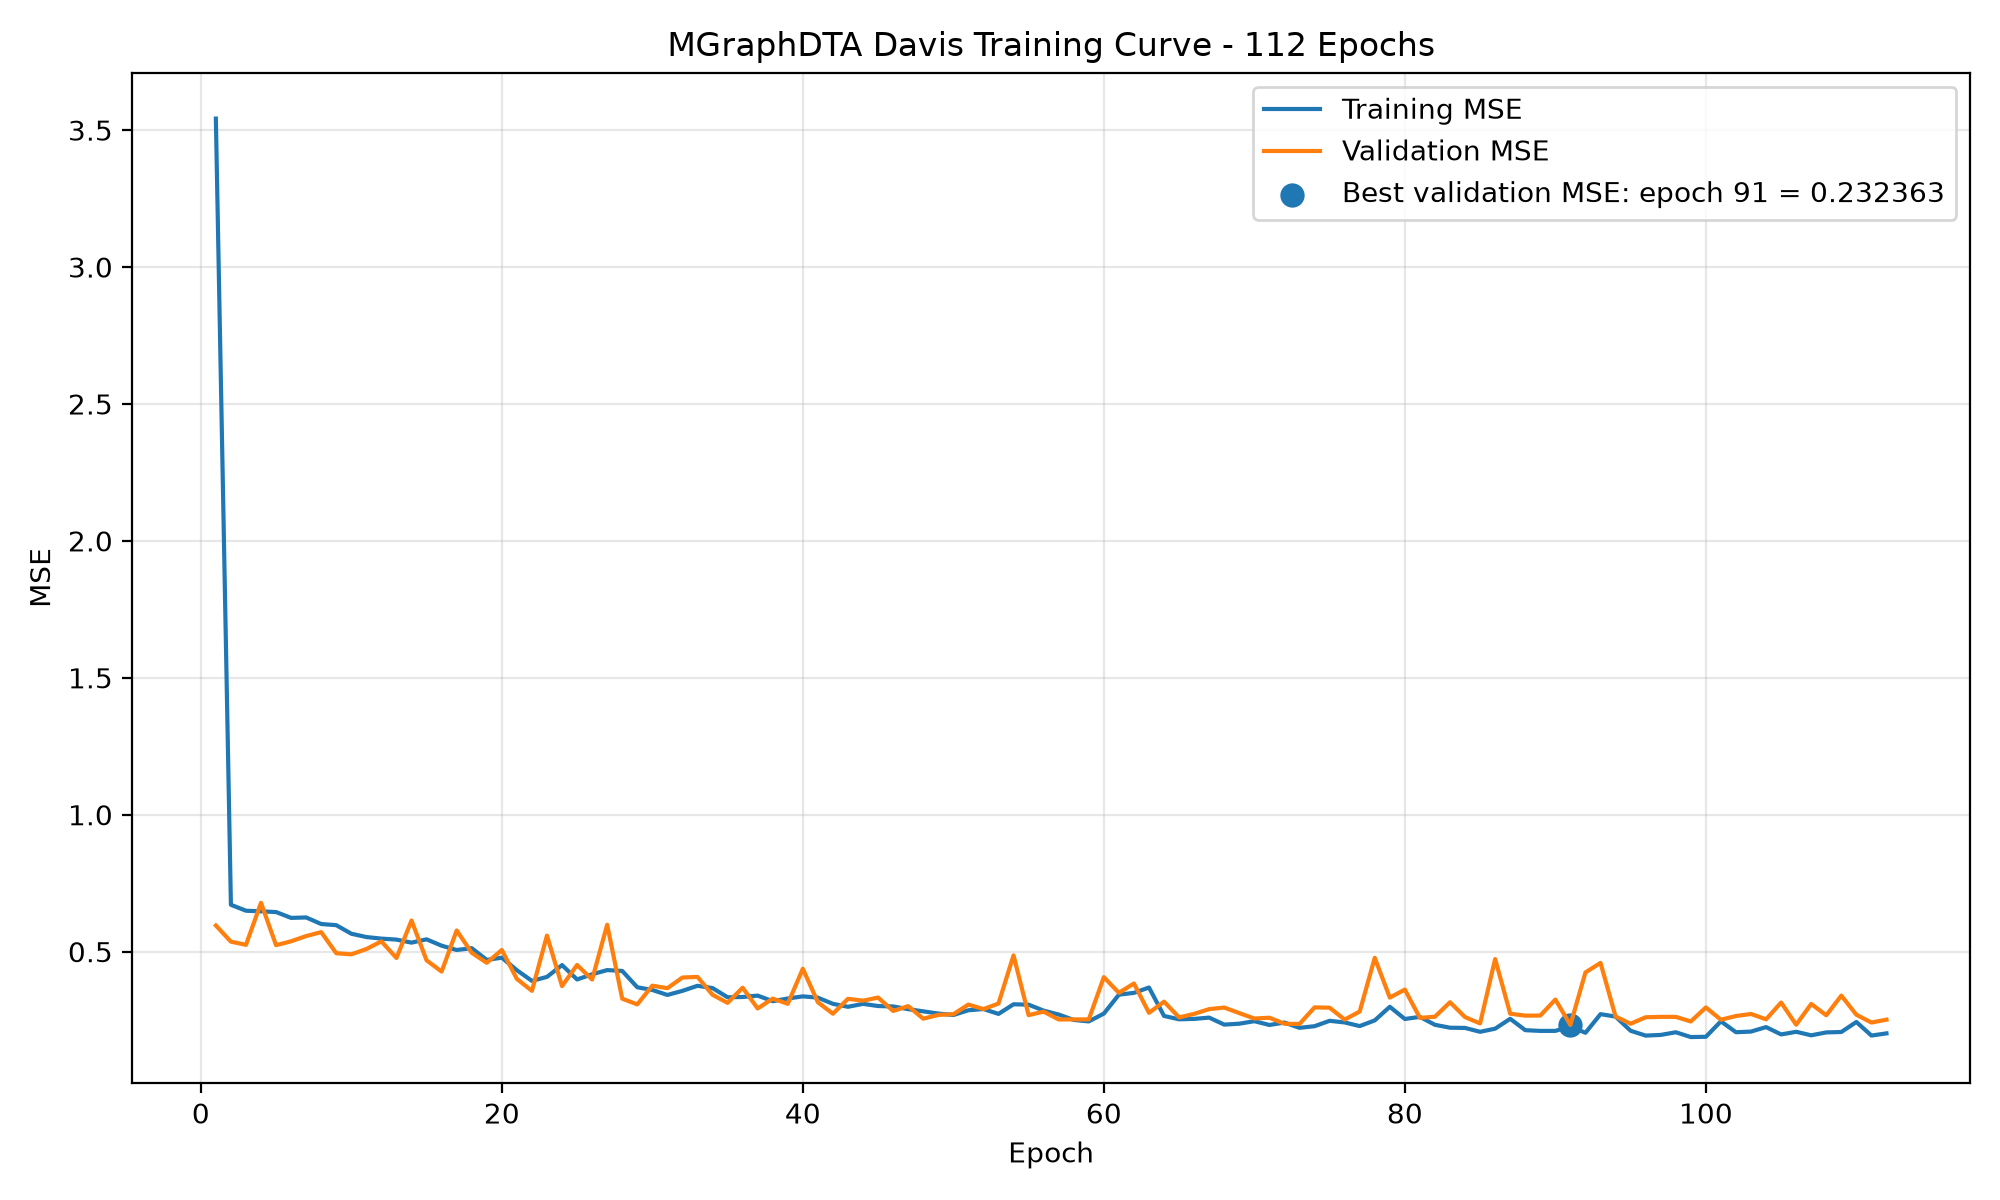
\includegraphics[width=0.9\linewidth]{figures/training_curve.png}\caption{Stored MGraphDTA training and validation MSE over 112 epochs. The best checkpoint is selected by validation MSE.}\label{fig:curve}\end{figure}
The best validation checkpoint, rather than the last epoch, is used for final test evaluation. The run was manually stopped at epoch 112; therefore the output does not establish a completed 150-epoch run.

\section{Project additions and changes}
\begin{longtable}{p{0.23\linewidth}p{0.33\linewidth}p{0.34\linewidth}}\caption{Verified implementation additions and their role}\label{tab:additions}\\\toprule Addition & What this project implements & Why it is useful / relation to paper\\\midrule\endfirsthead\toprule Addition & Implementation & Role\\\midrule\endhead
Independent test isolation & Test fold is loaded after best-checkpoint restoration and validation-based selection. & Makes the final test score independent of optimization and model selection in this pipeline; paper protocol differs.\\
Seed control & Seeds Python, NumPy, PyTorch and CUDA generators. & Supports repeatable split/initialization behavior; one run does not establish seed robustness.\\
Evaluation-only path & Stored checkpoint can be evaluated without training. & Separates scoring a chosen model from fitting.\\
Corrected $r_m^2$ & Formula in Eq.~\ref{eq:rm2}, covered by metrics tests. & Aligns with the authors' definition recorded in project docs; an earlier result JSON remains distinct.\\
Automated tests & Unit/integration tests cover the model and pipeline. & Checks shape, preprocessing, metric, attribution, and protocol invariants.\\
Grad-AAM & Atom attribution at \texttt{transition3}; five test examples saved. & Makes model sensitivity inspectable; attributions are not physical contacts.\\
Training records and curves & Epoch CSV, best checkpoint and PNG plot. & Preserves the observed optimization history and selection trace.\\
2D protein graph & Separate sequence-adjacency GNN and Davis run. & Explores a residue-node alternative; not part of main model.\\
Structural demonstrations & Five independent coordinate-based protein--ligand examples. & Gives concrete interaction-geometry examples, separate from Davis model outputs.\\
Documentation and organization & README, project plan, tests, scripts, results, checkpoints directories and repository history. & Makes the work navigable and the experiment traceable.\\\bottomrule\end{longtable}
These additions improve auditability and analysis; they are not claims that prediction accuracy was improved.

